\chapter{Dasar Teori}
\label{chap: dasarTeori}

\section{Sistem Informasi}
\label{sec: sistemInformasi}

	Sistem informasi adalah kombinasi dari teknologi informasi dan aktivitas orang yang menggunakan teknologi itu untuk mendukung operasi dan manajemen. Dalam arti yang sangat luas, istilah sistem informasi yang sering digunakan merujuk kepada interaksi antara orang, proses algoritmik, data, dan teknologi. 
	
	\subsection{Tujuan Sistem Informasi}
	\label{sub: tujuanSI}
	
		Tujuan dari sistem informasi adalah menghasilkan informasi. Sistem informasi adalah data yang diolah menjadi bentuk yang berguna bagi para pemakainya. Data yang diolah saja tidak cukup dapat dikatakan sebagai suatu informasi. Untuk dapat berguna, maka informasi harus didukung oleh tiga pilar sebagai berikut: tepat kepada orangnya atau relevan (\textit{relevance}), tepat waktu (timeliness), dan tepat nilainya atau akurat (\textit{accurate}). Keluaran yang tidak didukung oleh tiga pilar ini tidak dapat dikatakan sebagai informasi yang berguna, tetapi merupakan sampah (\textit{garbage}).
	
	\subsection{Komponen Sistem Informasi}
	\label{sub: komponenSI}
	
		Komponen prosedur dalam SI berkaitan dengan prosedur manual dan prosedur berbasis komputer serta standar untuk mengolah data menjadi informasi yang berguna. Suatu prosedur adalah urutan langkah yang dilakukan untuk menyelesaikan satu atau lebih aktivitas pengolahan informasi. Pengolahan informasi ini dapat dikerjakan dengan pengguna, atau kombinasi pengguna dan staff TI. Suatu bisnis terdiri dari berbagai macam prosedur yang digabungkan secara logis untuk membentuk suatu sistem. 
		
		SI dapat dikategorikan dalam empat bagian:
		
		\begin{enumerate}
			\item Sistem Informasi Manajemen
			\item Sistem Pendukung Keputusan
			\item Sistem Informasi Eksekutif
			\item Sistem Pemrosesan Transaksi
		\end{enumerate}
		
		\subsubsection{Sistem Informasi Manajemen}
		\label{subsub: SIManajemen}
		Sistem informasi manajemen atau SIM adalah sistem perencanaan bagian dari pengendalian internal suatu bisnis yang meliputi pemanfaatan manusia, dokumen, teknologi, dan prosedur oleh akuntansi manajemen untuk memecahkan masalah bisnis seperti biaya produk, layanan, atau suatu strategi bisnis. Secara akademis, istilah ini umumnya digunakan untuk merujuk pada kelompok metode manajemen informasi yang bertalian dengan otomasi atau dukungan terhadap pengambilan keputusan manusia, misalnya sistem pendukung keputusan, sistem pakar, dan sistem informasi eksekutif.
		
		\subsubsection{Sistem Pendukung Keputusan}
		\label{subsub: sistemPendukungKeputusan}
		Sistem pendukung keputusan adalah bagian dari sistem informasi berbasis komputer (termasuk sistem berbasis pengetahuan (manajemen pengetahuan)) yang dipakai untuk mendukung pengambilan keputusan dalam suatu organisasi atau perusahaan. 
		
		Tahapan SPK:
		\begin{enumerate}
			\item Definisi masalah
			\item Pengumpulan data atau informasi yang relevan
			\item Pengolahan data menjadi informasi baik dalam bentuk laporan grafik maupun tulisan
			\item Menentukan alternatif-alternatif solusi (bisa dalam persentase)
		\end{enumerate}
		
		\subsubsection{Sistem Informasi Eksekutif}
		\label{subsub: SIEksekutif}
		Sistem Informasi Eksekutif (EIS) adalah salah satu jenis manajemen sistem informasi untuk memudahkan dan mendukung keterangan dan pembuatan keputusan yang dibutuhkan eksekutif senior dengan menyediakan kemudahan akses terhadap informasi baik dari dalam maupun dari luar yang relevan dengan tujuan organisasi. Ini biasanya dipertimbangkan sebagai bentuk dari sistem pendukung keputusan (SPK).
		
		\subsubsection{Sistem Pemrosesan Transaksi}
		\label{subsub: sistemPemrosesanTransaksi}
		
		Sistem Pemrosesan Transaksi atau \textit{Transaction Processing System} adalah bagian dari sistem informasi yang merupakan sebuah sistem yang menjalankan dan mencatat transaksi rutin harian yang diperlukan untuk menjalankan bisnis. Contohnya adalah seperti memasukkan pesanan penjualan, pemesanan hotel,penggajian , pencatatan karyawan dan pengiriman. Tujuan utama dari sistem pada tingkat ini adalah untuk menjawab pertanyaan rutin dan melacak arus transaksi yang melalui organisasi.
		
\section{CodeIgniter}
\label{sec: codeigniter}

	\textit{CodeIgniter} merupakan sebuah \textit{framework} pemrograman \textit{web} dengan menggunakan bahasa php. \textit{CodeIgniter} (CI) akan membantu mengurangi jumlah pengerjaan kode yang harus diketik, mempermudah pembacaan dan pembaharuan \textit{script}, membantu penyusunan struktur yang jelas dan rinci, mendisiplinkan diri dalam pengerjaan \textit{coding} dan memperkuat hasil tanpa disadari.
	
	
	\subsection{Keistimewaan CI}
	\label{sub: KeistimewaanCI}
	CodeIgniter memiliki beberapa keistimewaan antara lain:
	\begin{enumerate}
		\item Menghemat waktu pengembangan
		\item \textit{Reuse of code} (pemakaian kembali kode yang sudah ada)
		\item Adanya bantuan dari komunitas CI
	\end{enumerate}	
	
	
	\subsection{Model, View, dan Controller(MVC) pada CI}
	\label{sub: mvc}
	
	Konsep MVC adalah konsep pemisahan antara logic dengan tampilan dan database. Manfaat konsep ini adalah, membuat coding logic lebih simple, karena sudah di pisah dengan code untuk tampilan dan membuat programmer dapat bekerja secara terpisah dengan designer.
	CodeIgniter sendiri dibangun menggunakan konsep \textit{Model-View-Controller development pattern}. Manfaat konsep MVC ini adalah memudahkan logika dalam \textit{coding} aplikasi tersebut dan memudahkan pengembangan sistem yang sudah ada.
	\begin{itemize}
		\item \textit{Model} = \textit{Model} berhubungan dengan data dan interaksi ke \textit{database} atau \textit{webservice}. \textit{Model} juga merepresentasikan struktur data dari aplikasi yang bisa berupa basis data maupun data lain, misalnya dalam bentuk file teks, \textit{file} XML maupun webservice. Biasanya di dalam model akan berisi class dan fungsi untuk mengambil, melakukan update dan menghapus data website. Sebuah
		aplikasi web biasanya menggunakan basis data dalam menyimpan data, maka pada bagian \textit{Model} biasanya akan berhubungan dengan perintah-perintah \textit{query} SQL.
		\item \textit{View} = \textit{View} berhubungan dengan segala sesuatu yang akan ditampilkan ke \textit{end-user}. Bisa berupa halaman web, rss, javascript dan lain-lain. Di dalam \textit{view} hanya berisi variabel-variabel yang berisi data yang siap ditampilkan. View dapat dikatakan sebagai halaman website yang dibuat dengan	menggunakan HTML dan bantuan CSS atau JavaScript. \textit{View} hanya dikhususkan untuk menampilkan data-data hasil dari \textit{model} dan \textit{controller}
		\item \textit{Controller} = \textit{Controller} bertindak sebagai penghubung data dan \textit{view}. Di dalam \textit{Controller} inilah terdapat kelas-kelas dan fungsi-fungsi yang memproses permintaan dari View ke dalam struktur data di dalam \textit{Model}. \textit{Controller} juga tidak boleh berisi kode untuk mengakses basis data karena tugas mengakses data telah diserahkan kepada \textit{model}. Tugas \textit{controller} adalah menyediakan berbagai variabel yang akan ditampilkan di \textit{view}, memanggil \textit{model} untuk melakukan akses ke basis data, menyediakan penanganan kesalahan/\textit{error}, mengerjakan proses logika dari aplikasi serta melakukan validasi atau cek terhadap \textit{input}.
	
	\end{itemize}
	
	Berikut ini adalah alur proses konsep MVC:
	
	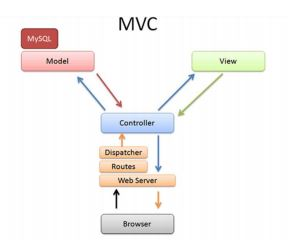
\includegraphics[scale=1.00]{Gambar/konsepMVC}
	
	CI menerapkan pola MVC yang flexible, karena model dapat tidak di gunakan. Anda dapat hanya menggunakan Controller dan View saja dalam menggunakan CI
	tanpa Model. Jika anda tidak memerlukan pemisahan di dalam struktur data dan database atau menganggap penggunaan model hanya menambah kompleks aplikasi dengan keuntungan yang kurang sebanding, maka anda dapat tidak menggunakan model.
	
	\subsection{Struktur CI}
	\label{sub: strukturCI}
	CI adalah sebuah php framework yang berupa kumpulan folder dan file php, java script,css,txt dan file berbasis web lainnya dengan setting tertentu untuk menggunakannya dan menyediakan library dan helper yang dapat di manfaatkan di dalam pemrograman php. CI di jalankan under web dan harus dengan web server. Program CI cukup di letakkan di bawah folder directory web server anda.
	Berikut adalah struktur file CI :
	
	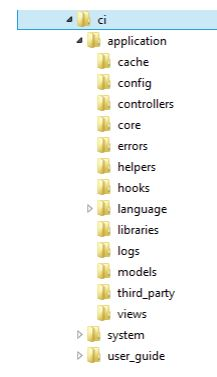
\includegraphics[scale=1]{Gambar/strukturCI}
		

\section{AngularJS}
\label{sec: angularJS}
	
	AngularJS merupakan \textit{framework javascript} berbasis \textit{open-source} yang dirilis oleh Google pada tahun 2009. AngularJS sendiri merupakan jawaban dari banyak tantangan pemakaian web yang memerlukan pengaplikasian suatu fungsi tanpa berganti halaman. Jika anda merujuk pada situs resmi AngularJS yaitu http://angularjs.org maka anda akan dapat membaca sebuah tagline "HTML Enchanced for Web Apps". Tag line tersebut mengartikan bahwa pemakaian angularJS merupakan pemakaian HTML yang telah ditingkatkan fungsinya untuk membangun sebuah aplikasi dalam web.
	
	HTML merupakan alat yang digunakan untuk membangun web statik sehingga membutuhkan bantuan dari alat lain untuk membuat sebuah aplikasi web pada HTML ini. Oleh sebab minat dan banyaknya permintaan dari developer web untuk membuat aplikasi web dengan mudah, maka Google meresmikan AngularJS pada tahun 2009 yang lalu.
	
	AngularJS bukan merupakan pustaka (\textit{library}) javascript melainkan sebuah framework yang solid untuk membangun web app, seperti \textit{framework} javascript pada umumnya AngularJS mengadopsi konsep MVC (\textit{Model}, \textit{View}, \textit{Controller}), meskipun menggunakan implementasi yang berbeda dengan konsep asli MVC.
	
\subsection{Keistimewaan AngularJS}
\label{sub: keistimewaanAngularJS}
	Berikut beberapa keistimewaan dari pemakaian AngularJS:
	
\subsubsection{Two way data-binding}
\label{sub: twoWayDataBinding}

	\textit{Two way data-binding} merupakan mekanisme sinkronisasi otomatis antara \textit{Controller} dan \textit{View}. Ketika ada perubahan pada \textit{Model} yang berasal dari \textit{View}, AngularJS secara otomatis membuat perubahan pada \textit{Controller}. Begitu pula sebaliknya. Hal ini terjadi secara otomatis, jadi tidak diperlukan penulisan kode secara manual untuk mencapai mekanisme tersebut.

\subsubsection{HTML Template}
\label{subsub: HTMLTemplate}

	\textit{Template} yang digunakan AngularJS hanyalah HTML biasa dengan penambahan ekspresi (\textit{expression}), sehingga tidak diperlukan penggunaan \textit{template engine} khusus.

\subsubsection{Dependecy Injection (DI)}
\label{subsub: DI}

	\textit{Dependency Injection} memungkinkan \textit{developer} menulis beberapa komponen kode yang terpisah satu sama lain. Ketika memerlukan salah satu komponen, \textit{developer} dapat melakukan pemanggilan komponen yang dibutuhkan dan dapat menggunakan fungsi komponen tersebut. Fitur ini memudahkan \textit{developer} dalam membuat komponen yang dapat dipakai berulang kali (reusable component)

\subsection{Komponen AngularJS}
\label{sub: komponenAngularJS}
	


\subsubsection{Model}
\label{subsub: model}

	Dalam pola MVC, \textit{Model} merepresentasikan suatu set data yang digunakan oleh \textit{Controlle}r dan \textit{View}. \textit{Model} dapat mendeteksi perubahan data dan memberikan notifikasi perubahan tersebut ke \textit{Controller} dan \textit{View}. Untuk membuat \textit{Model} di beberapa framework selain AngularJS diperlukan konstruktor khusus, sedangkan \textit{Model} pada AngularJS tidak memiliki konstruktor tersendiri dan tidak memerlukan pemanggilan fungsi \textit{inheritance} dari \textit{Object Class} tertentu, tidak memerlukan metode \textit{setter} atau \textit{getter} khusus, dan bisa berupa \textit{primitive}, \textit{object hash}, atau \textit{full object} yang berarti \textit{Model} hanyalah javascript \textit{object} biasa.

\subsubsection{Scope}
\label{sub: Scope}

	\textit{Scope} merupakan perekat (\textit{glue}) atau perantara antara \textit{Controller} dengan \textit{View}. Masing-masing \textit{controller} memiliki \textit{scope} atau lingkup masing - masing.
	
\subsubsection{Controller}
\label{subsub: controller}

	\textit{Controller} merupakan kode dibalik \textit{View}. Isi dari \textit{controller} merupakan kode pemrosesan dan logika yang akan menghasilkan \textit{Model} untuk ditampilkan pada \textit{View}.

\subsubsection{View}
\label{subsub: view}

	\textit{View} adalah apa yang terlihat oleh pengguna, yang dimulai dari sebuah \textit{template}, digabungkan dengan \textit{Model}, dan \textit{browser} melakukan proses \textit{rendering} hingga hasil keseluruhan proses tersebut ditampilkan ke pengguna. \textit{Template} yang digunakan hanyalah sintak HTML (bukan HTML diselingi dengan \textit{markup} khusus seperti pada template engine pada umumnya).

\subsubsection{Expression}
\label{subsub: expression}

	\textit{Expression} merupakan kode \textit{snippet} yang dapat kita tulis pada \textit{View}. \textit{Expression} berkaitan dengan mekanisme \textit{binding} pada AngularJS, formatnya adalah sebagai berikut \{\{ expression \}\} Contoh :
	
	\begin{enumerate}
		\item "\{\{ 1+2 \}\}" , akan menampilkan angka 3 ke pengguna.
		\item \{\{ user.name \}\} , akan menampilkan nilai properti 'name' dari model 'user'
		\item \{\{ 1000 | currency \}\} , akan menampilkan angka 1000 dalam format mata uang (currency), keyword setelah tanda pipa ( | ) merupakan filter.
	\end{enumerate}

\subsubsection{Directive}
\label{subsub: directive}

	\textit{Directive} merupakan cara untuk membuat sintak HTML baru yang akan dimengerti oleh \textit{browser}. \textit{Directive} dapat berupa elemen, \textit{attribute}, \textit{HTML comment} atau \textit{Class}. Angular telah menyediakan beberapa \textit{directive} bawaan yang penting dalam pengembangan aplikasi berbasis \textit{web}. Beberepa \textit{directive} bawaan Angular diantaranya adalah ng-controller, ng-model, ng-repeat, ng-click.
	
\section{Twitter Bootstrap}
\label{sec: bootstrap}

	Twitter Bootstrap adalah sebuah alat bantu untuk membuat sebuah tampilan halaman \textit{website} yang dapat mempercepat pekerjaan seorang pengembang \textit{website} ataupun pendesain halaman \textit{website}. Sesuai namanya, website yang dibuat dengan alat bantu ini memiliki tampilan halaman yang sama / mirip dengan tampilan halaman \textit{Twitter} atau desainer juga dapat mengubah tampilan halaman \textit{website} sesuai dengan kebutuhan.

	Twitter Bootstrap dibangun dengan teknologi HTML dan CSS yang dapat	membuat layout halaman website, tabel, tombol, form, navigasi, dan komponen	lainnya dalam sebuah website hanya dengan memanggil fungsi CSS (class) dalam berkas HTML yang telah didefinisikan. Selain itu juga terdapat komponen-komponen lainnya yang dibangun menggunakan JavaScript.
	
	\subsection{Struktur direktori Bootstrap}
	\label{sub: struturDirektoriBootstrap}
	
	Berikut adalah gambar struktur direktori dari \textit{Bootstrap}:
	
	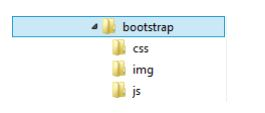
\includegraphics[scale= 1.0]{Gambar/strukturBootstrap}
	
	\subsection{Keuntungan menggunakan Bootstrap}
	\label{sub: keuntunganBootstrap}
	
	Penggunaan \textit{Twitter Bootstrap} tentu saja memiliki banyak keuntungan, diantaranya adalah:
	
	\begin{itemize}
		\item Memudahkan dalam mendesain website
		\item Responsif (mendukung segala macam layar dan \textit{device})
		\item Adanya dokumentasi yang cukup lengkap
		\item Mempunyai tampak yang elegan
	\end{itemize} 
	
	